
%%%%%%%%%%%%%%%%%%%%%%%%%%%%%%%%%%%%%%%%%%%%%%%%%%%%%%%%%%%%%%%%%%%%%%%%%%%%%%%%%%%%%%%%%%%%%%%%
% Biodiversity
%%%%%%%%%%%%%%%%%%%%%%%%%%%%%%%%%%%%%%%%%%%%%%%%%%%%%%%%%%%%%%%%%%%%%%%%%%%%%%%%%%%%%%%%%%%%%%%%


\chapter{FLR impacts on biodiversity\label{ch:biodiv}} 

Due to the severe degradation of ecosystems by human activities (e.g. land clearing, fragmentation), the persistence and representation of several species currently depend not only on habitat protection, but also on habitat restoration \citep{Crouzeilles2015}. Restored ecosystems should meet two  conservation objectives for biodiversity: representativeness and persistence \citep{NossReedNielsenScottVance-Borland1982}. The first objective claims that restored ecosystems should be representative of the variety of populations, species and ecosystem functions within each region, while the second aims to guarantee the long-term persistence of these elements in the landscape \citep{Margules2000}. Both objectives depend on processes related with the (re)coloniza-tion, supplementation and maintenance of wildlife species and populations in restored systems and surrounding landscapes \citep{Helmer2008, Crk2009, Crouzeilles2016a}. Here we quantified these processes in terms of biodiversity restoration, species connectivity and species extinction risk. 
%
%-----------------------------------------------------------------------------------------------
\section{\Large Biodiversity restoration}\label{sec:bio-recov}
\subsection{\large Biodiversity restoration using different restoration methods} \label{subsec:bio-revisão}
%
There is an increasing global understanding of biodiversity restoration patterns within two key types of restoration methods: active restoration and natural regeneration (also referred as passive restoration) (e.g. Crouzeilles \cite{Crouzeilles2017a}; Box\ref{Box2}), but we know little on how it applies to specific biomes. Aiming to understand how restoration has impacted biodiversity conservation and climate change mitigation (section \ref{ch:carbon}), we have conducted a literature review on studies on the impacts of different restoration methods on biodiversity and carbon stocks in Brazil. We conducted a systematic literature review searching the databases Scopus, Web of Science, Science Direct, Scielo and Periódicos Capes for published articles, using Boolean searches with the word strings Carbon* OR Biomass OR Biodiversity OR Diversity OR Richness AND restorat* OR natural regeneration OR succession OR Agroforest* in the abstract, title or keywords. We repeated the search in English and in Portuguese. During each search we selected relevant articles based on the abstract and keywords, totaling 202 articles that were included in our literature database using the Mendeley software. \\
\indent Intending to perform a quantitative comparisons (meta-analysis) on how different restoration methods affects biodiversity and carbon stocks (section \ref{ch:carbon}), we have further selected articles according to the following criteria: (i) must provide data on a restoration area (active or passive restoration, agroforest system or silviculture); (ii) must have an original (e.g. a mature or old-growth forest) or negative reference area (e.g. a degraded area or pasture or agricultural land); (iii) must have measured biodiversity and/or carbon and/or biomass stocks in the soil, above and/or belowground components. Such selection has eliminated 92 studies that were out of scope (41 articles, 44\%), did not have a reference ecosystem (36 articles, 39\%), lacked basic information (11, 12\%), or were based on the same data used in another article already included (4, 4\%). We have then retained 110 articles, from which we have already extracted the relevant information to perform the meta-analysis. We extracted information on 44 indicators including location, restoration method, species used, biome, vegetation type, previous land use history, restoration age, pre and post planting management, sample size and mean and variance values for biodiversity and/or carbon and/or biomass metrics from any compartment. Many articles provide poor description on their experimental design and/or do not provide mean and standard deviation values in tables, so when necessary we extracted data from graphs using an image tool (https://automeris.io/WebPlotDigitizer/). We then calculated the standardized mean difference (response ratio) between the biodiversity or carbon values from each restored area and the reference ecosystems (being an original or negative reference). The compiled dataset already been checked and standardized and is ready for the next step of performing the statistical analyses. \\
\indent Results show that the knowledge on ecological restoration in Brazil is concentrated on forest biomes, being mainly based on the Atlantic forest (63\% of the compiled studies, 69 studies), followed by the Amazon (26\%, 29 studies) (Figure \ref{fig:Bio-Cata-1} A). The restoration method of passive restoration was the most studied in both forest biomes (Figure \ref{fig:Bio-Cata-1} C) probably due to the longest history of studies on secondary forest succession than on active restoration (Figure \ref{fig:Bio-Cata-1} B). Most studies compared the areas under restoration with an original reference and only a few had a negative reference (Figure \ref{fig:Bio-Cata-1} D).  
%
%%%%%% FIgura CATA 1 A-D %%%%%%%% 
\begin{figure}[H]
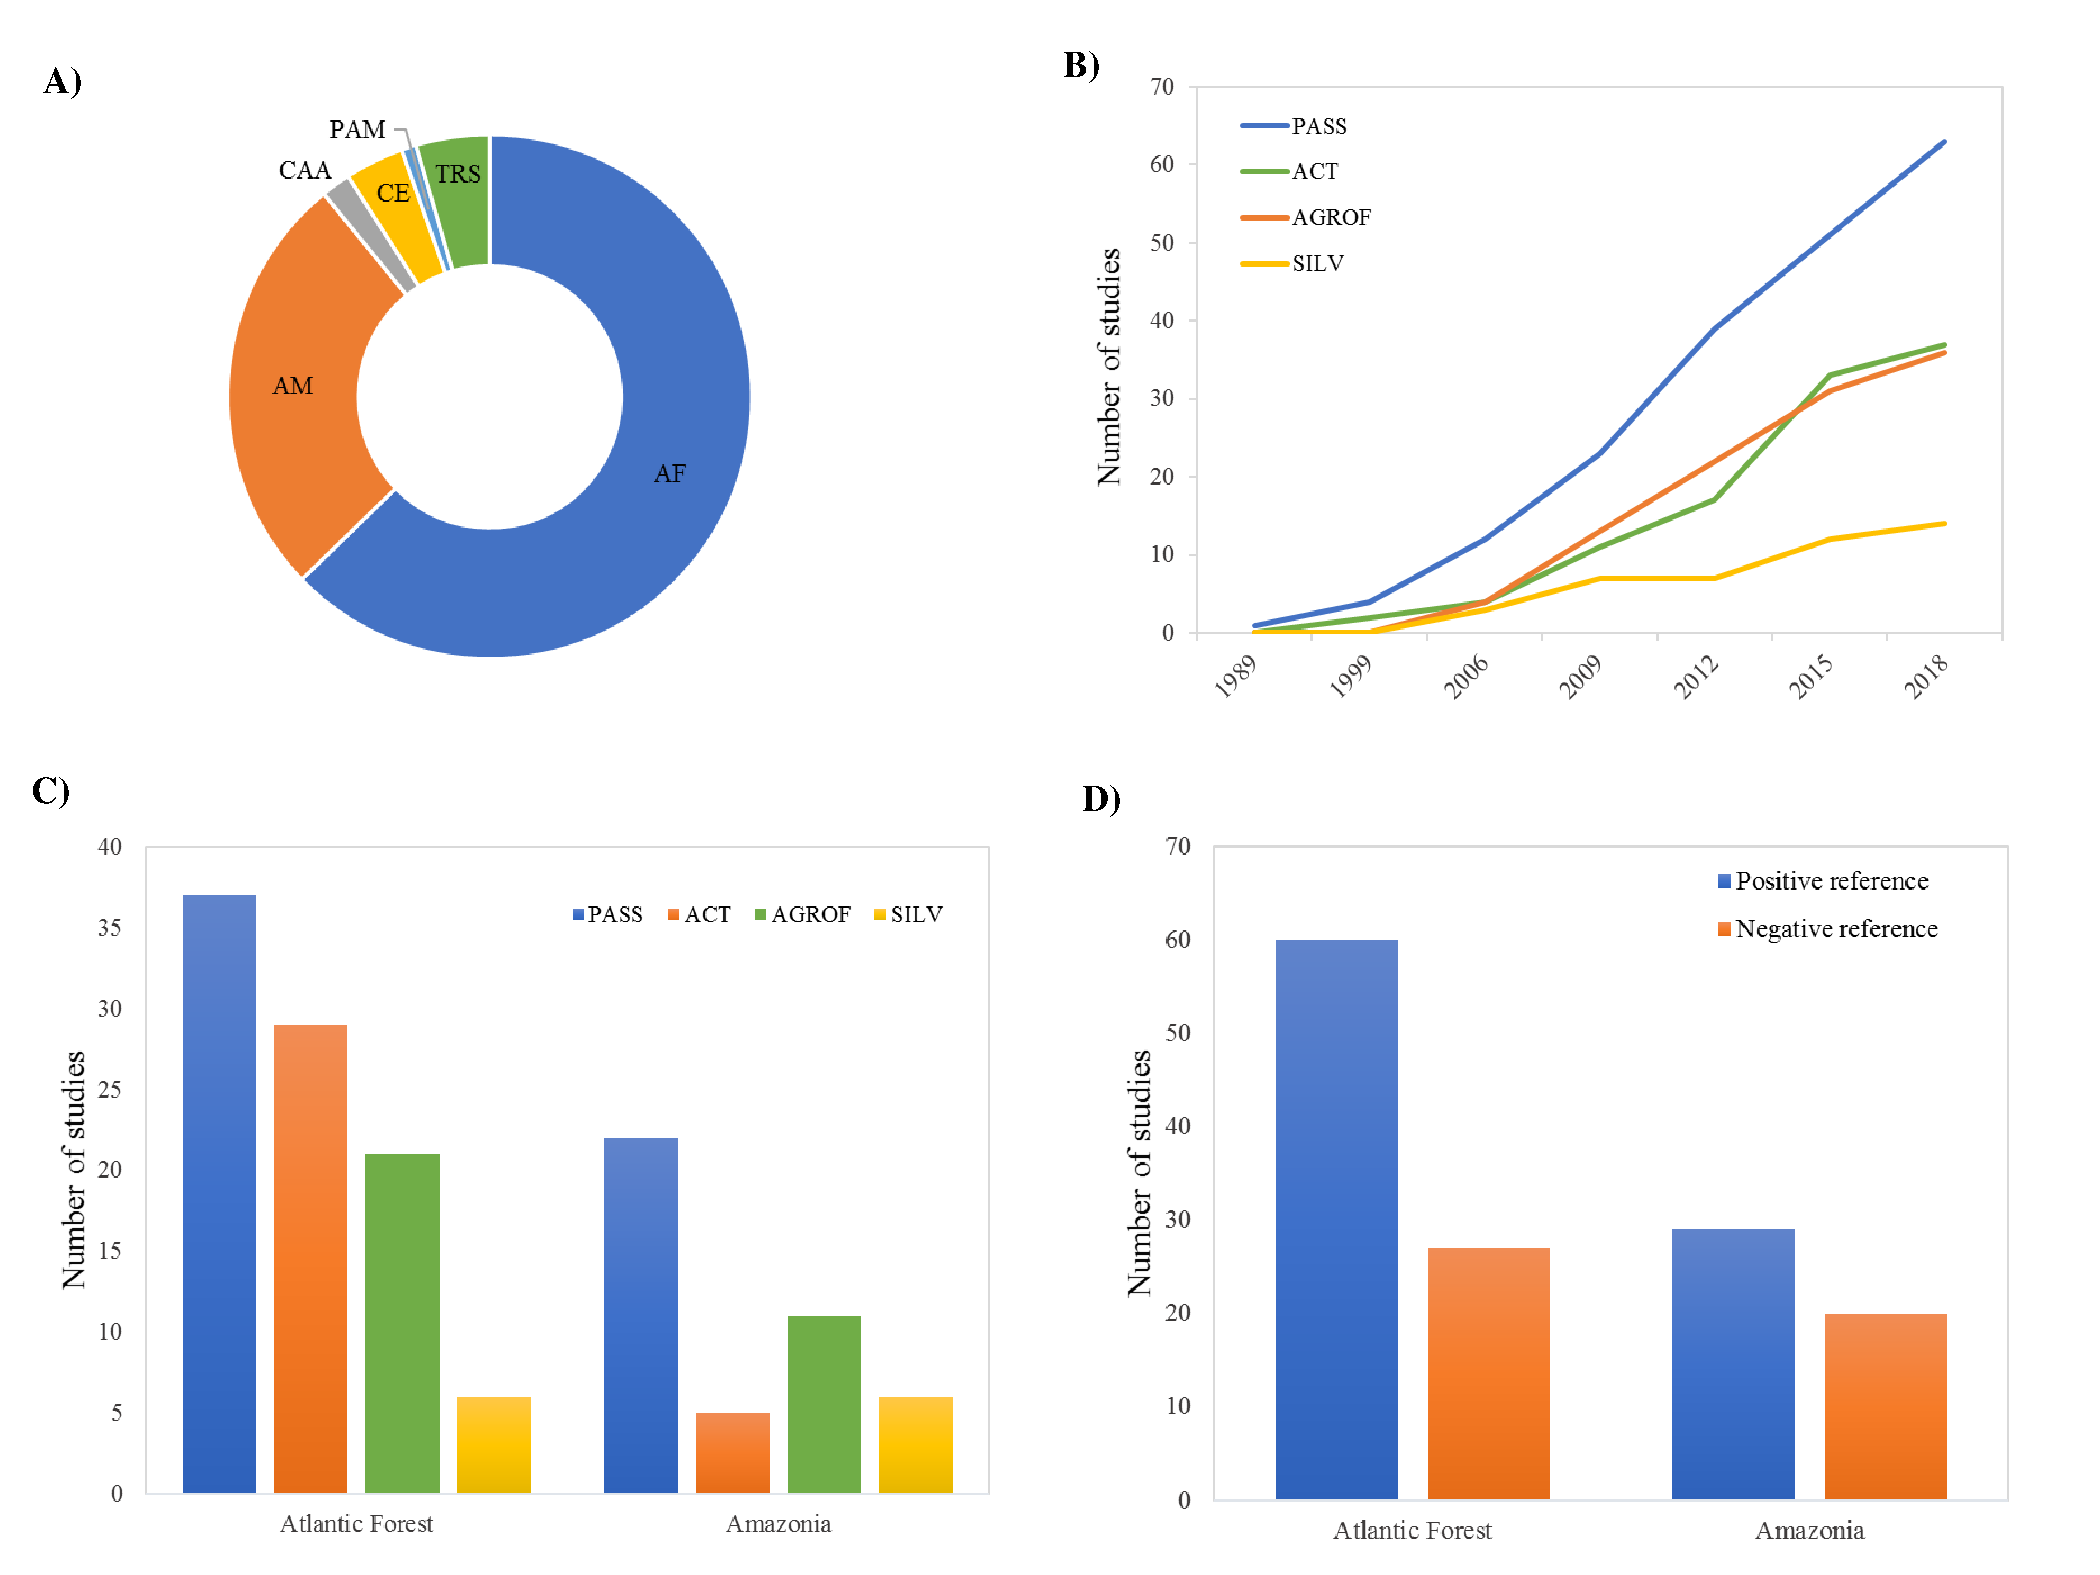
\includegraphics[width=1.0\linewidth]{pictureve/Bio-Cata-1.pdf}
\caption{(A) Proportion of the compiled studies in each Brazilian biome (AF-Atlantic forest, AM-Amazon, CAA-Caatinga, CE-Cerrado, PAM-Pampa, TRS-Transition between Cerrado and Atlantic Forest or Amazon); (B) Number of studies on the different restoration methods (Passive, Active, Agroforestry, Silviculture) over time; (C) Number of selected studies including each restoration technique in the Atlantic Forest and Amazon; (D) Number of selected studies including a positive or negative reference (some studies had both).}
\label{fig:Bio-Cata-1}
\end{figure}
%

\newpage
Among the 98 studies done in the forest biomes, 79 included some type of biodiversity measure, being 49 and 22 in the Atlantic Forest and Amazon, respectively (Figure \ref{fig:Bio-Cata-2}). As one study may have included more than one biome, the total number of studies available for our meta-analysis is 66 and 28 for the Atlantic Forest and Amazon, respectively. Most selected studies focused on animals followed by plants and soil biology (Figure \ref{fig:Bio-Cata-2}). Although the higher amount of studies on animals than on plants seems unexpected, other meta-analysis found the same pattern in a global scale (e.g. Crouzeilles \citep{Crouzeilles2017a}). Species richness was the most used biodiversity measure (35 and 16 in the Atlantic Forest and Amazon, respectively), while species composition (similarity between restored and natural ecosystems) was the least used metric, only present in 13 studies (8 and 5 in the Atlantic Forest and Amazon).

%
%%%%%% FIgura CATA 2 %%%%%%%%
\begin{figure}[H]
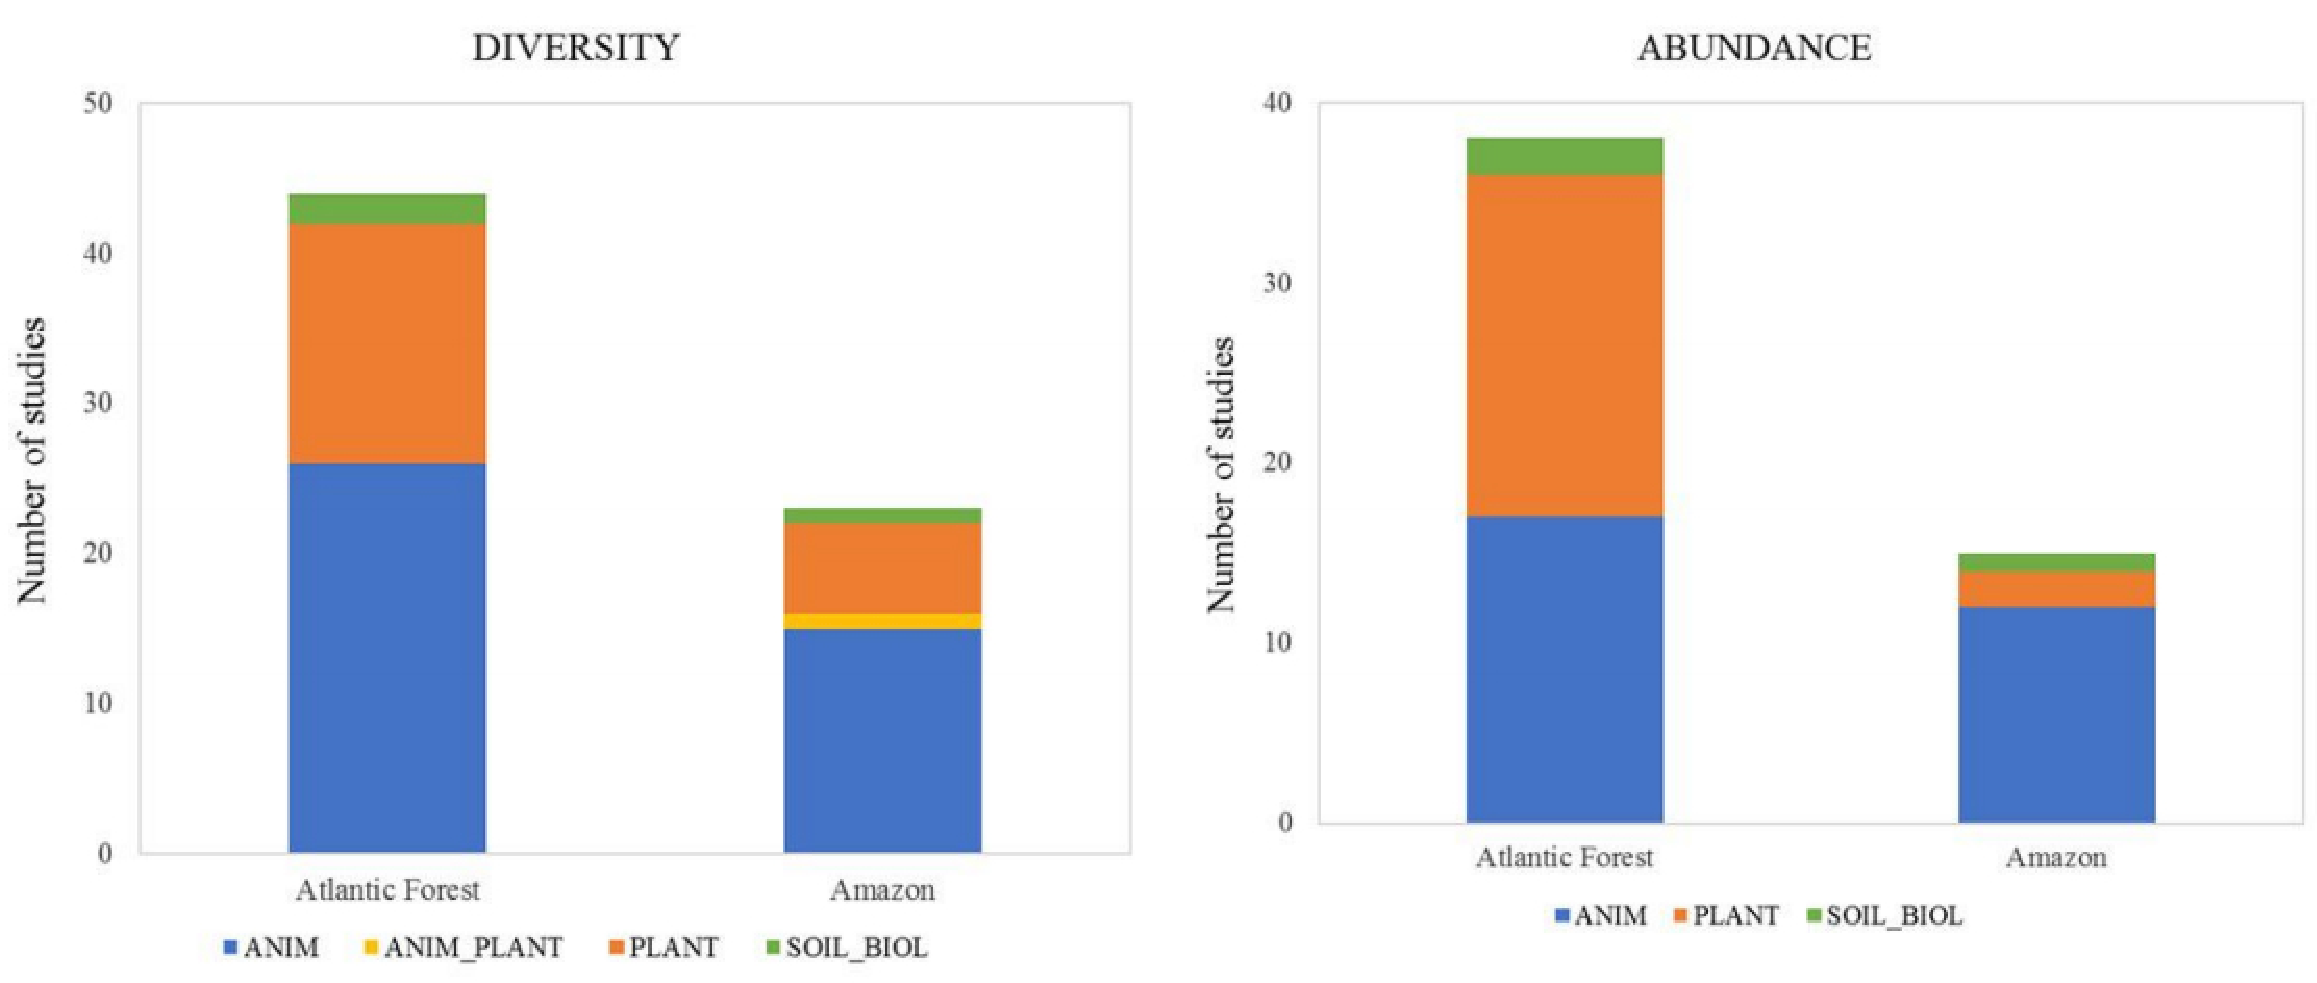
\includegraphics[width=1.0\linewidth]{pictureve/Bio-Cata-2.pdf}
\caption{Number of studies that analyzed the effects of restoration on the biodiversity (A) and abundance (B) in the Brazilian Atlantic Forest and Amazon biomes, and the proportion of studies on animals (ANIM), plants (PLANT), animal-plant together and soil fauna (SOIL-BIOL).}
\label{fig:Bio-Cata-2}
\end{figure}

\newpage
%
%%%% Box tipos de restauracao
\begin{center}
\begin{mybox}{Definitions of actively and passively restored systems, simplified and biodiverse agroforestry systems, degraded and reference systems}
\label{Box2}
{\bf Negative reference:} Agricultural monoculture plantations and monoculture planted forests or pastures, that is, conventional production systems \citep{Crouzeilles2016a}.
%
{\bf Restored systems:} Selectively logged forests or forests in their initial or secondary stage of succession, that is, areas that regenerated after complete or partial clearance \citep{Crouzeilles2016a}. 
    {\bf Passive restoration (or natural regeneration) systems:} Forest regrowth following land abandonment, selective logging or assisted recovery of native tree species through human interventions, such as fencing, to control livestock grazing, weed control, and fire protection \citep{Shono2007, Zahawi2014, Crouzeilles2017a}.
    {\bf Active restoration systems:} Manipulating disturbance regimes through the use of thinning and burning, the establishment of nursery-grown seedlings, direct seeding, or plantations of tree species \citep{Shono2007, Zahawi2014, Crouzeilles2017a}.
%
{\bf Original reference:} Old-growth or less-disturbed forests \citep{Crouzeilles2016a}
%
{\bf Agroforestry systems:} Land management practice where trees, shrubs, agricultural crops, and animals are used simultaneously or sequentially to produce a large range of products such as timber, fiber, fruits, nuts, annual crops, medicinal plants, and oils (OTS/CATIE, 1986, \cite{May2008} . Simple and biodiverse agroforestry systems were classified according to well-established criteria related to the vegetation structure (density, number of layers, and management dynamics), cultivated species richness, and complexity of interactions over time and space \citep{Schroth2004, Steenbock2003, MiccolisAndrewPeneireiroFabianaMongeliMarquesHenriqueRodriguesVieiraDanielLuisMasciaArco-VerdeMarceloFrancioHoffmannMauricioRigonRehderTatianaPereira2016}.
    {\bf Simple agroforestry systems:} Less than five species; up to three layers (often dominant, intermediate, and live coverage); may or may not use native species, and crops are usually planted in alley cropping or rows; and not based on the local ecosystem and ecological succession.
    {\bf Biodiverse agroforestry systems:} Five or more species; more than three layers (generally divided into short, medium, tall, and emergent); based on local ecosystems, which use indigenous local species and exotic species that are similar in ecological function; and uses the local ecological succession throughout the years as a principle, associated with management dynamics and production staggered over time  \cite{Santos2019}.
\end{mybox}
\end{center}

\newpage
%%%%%%%%%%%%%%%%%%%%%%%%%%%%%%%%%
\subsection{\large Biodiversity restoration in agroforestry systems} \label{subsec:bio-recovery-SAF} 

Few studies have quantified the capacity of agroforestry systems to conserve biodiversity. Agroforestry systems have been recommended as a cost-effective strategy that integrates production and biodiversity conservation, and as a restoration method. Under the NVPL, restoration with agroforestry systems is allowed in Legal Reserves and in Permanent Preserved Areas inside small rural properties (over 4 fiscal modulates). There are, however, different types of agroforestry systems \citep{ MiccolisAndrewPeneireiroFabianaMongeliMarquesHenriqueRodriguesVieiraDanielLuisMasciaArco-VerdeMarceloFrancioHoffmannMauricioRigonRehderTatianaPereira2016} which may contribute differently to biodiversity conservation and to ecosystem restoration. \\
\indent We compared values of different ecological metrics for biodiversity (species richness, abundance, diversity and/or similarity) within simplified and biodiverse agroforestry systems, negative reference systems and original reference systems in the Atlantic Forest \citep{Santos2019}. Values of biodiversity recovery were always lower in agroforestry and degraded systems compared to original reference systems (Figure \ref{fig:Bio-Renatinho-1}). Nonetheless, biodiversity recovery was 15\% and 45\% higher in biodiverse agroforestry systems than in simplified agroforestry systems and negative reference systems, respectively. Simplified agroforestry systems had higher values of biodiversity recovery (30\%) than degraded systems. \\
\indent Our results show that agroforestry systems do not result in similar values of biodiversity to those found in old-growth and less-disturbed forests (i.e. full recovery), corroborating the idea that primary forests are indeed irreplaceable for the maintenance of biodiversity \citep{Gibson2011, Crouzeilles2016a}. Agroforestry systems, however, hold significantly higher levels of biodiversity restoration than simplified monocultures, indicating the potential to complement biodiversity conservation and restoration in FLR initiatives. We also found that the type of agroforestry system is critical to determine biodiversity restoration, with biodiverse agroforestry systems recoverying higher levels than simplified agroforestry systems. Combined, these results indicate that biodiverse agroforestry systems may, over long periods of ecological succession, promote the restoration of biodiversity in rural landscapes and should be considered as an alternative restoration method to restore degraded lands in human-modified landscapes that can reconcile sustainable production and biodiversity conservation. 

\newpage
%%%%%% FIgura Bio-Renatinho 1 %%%%%%%%
\begin{figure}[H]
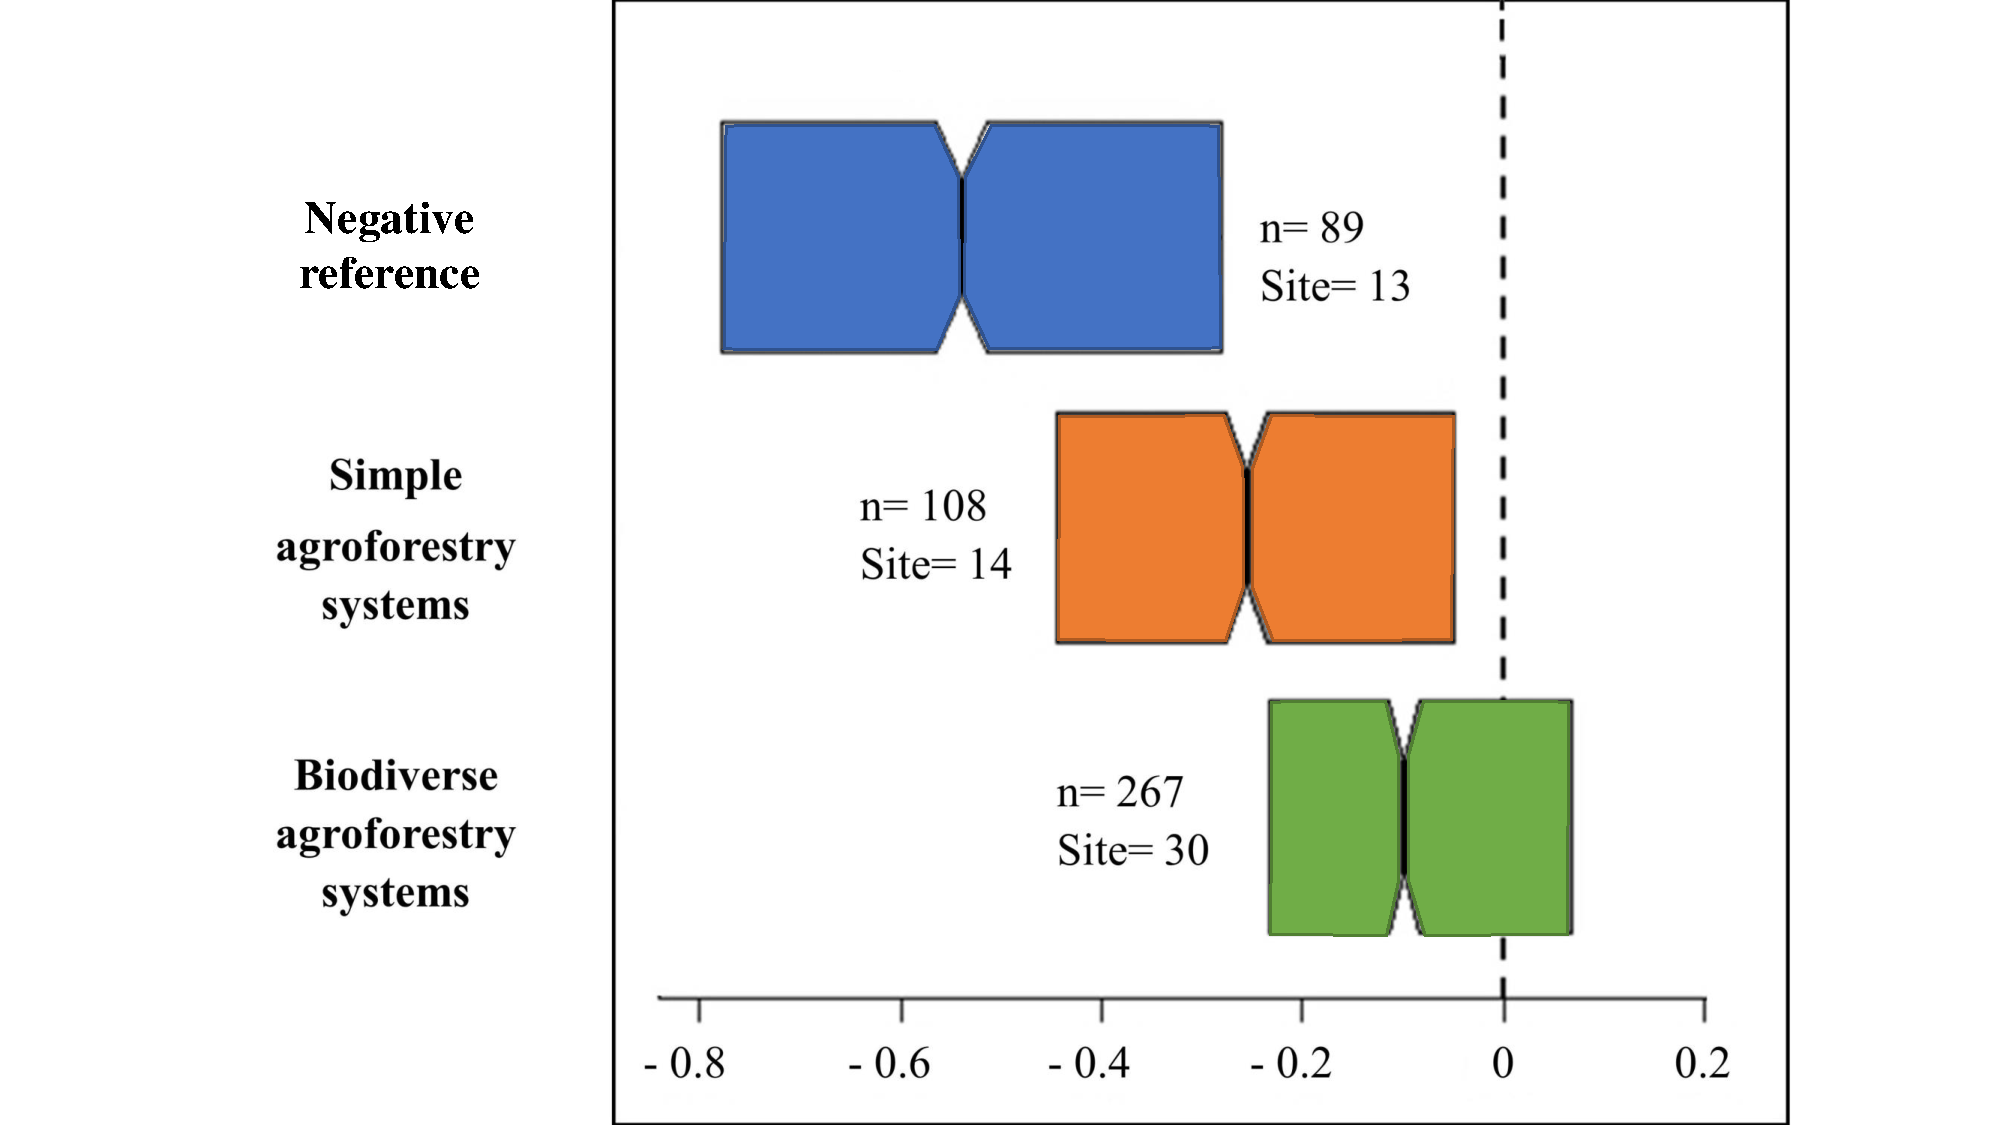
\includegraphics[width=1.0\linewidth]{pictureve/Bio-Renatinho-1.pdf}
\caption{Values of biodiversity recovery for negative reference systems, simple and biodiverse agroforestry systems compared to original reference systems in the Brazilian Atlantic Forest. Negative values (measured as median effect size) means that biodiversity recovery in restored/agroforestry/negative reference systems did not reach a benchmark state yet when compared to original reference systems. The opposite holds for positive values: values of biodiversity in restored/agroforestry/negative reference systems surpasses those found in reference systems. Values around zero are the desired outcome of restoration: when restored/agroforestry/negative reference systems have reached a benchmark level. Dashed lines indicate no significant difference with reference systems. n = sample size, site = number of study landscapes. The box plots show the mean effect size, and the variation of the first and third quartile of resampled response ratios. Notches (triangles) in the boxes represent 95\% confidence intervals and non-overlapping notches between boxes imply a significant difference \citep{Crouzeilles2016a}.}
\label{fig:Bio-Renatinho-1}
\end{figure}


%-----------------------------------------------------------------------------------------------

\section{\Large Landscape connectivity }\label{sec:bio-connect}

In order to allow for effective biodiversity recovery in restored and agroforestry systems, native and restored ecosystems must be connected within landscapes \citep{Crouzeilles2014, Crouzeilles2015}. Landscape connectivity is the degree to which the landscape facilitates or impedes species movements among habitat patches. %(Tayler et al. 1993) Nao estava nas referencias!. 
Landscape connectivity minimizes the effects of habitat loss and fragmentation on biodiversity and improves gene flow, wildlife dispersal, population viability and ecosystem services \citep{Lindenmayer2006, Galpern2011}. The effectiveness of landscape connectivity for biodiversity depends on habitat quality, amount and configuration of the habitat within a landscape, and species dispersal ability. Connectivity, therefore, varies among species in the same landscape, and for the same species among landscapes \citep{CROUZEILLES2013}. 

We used a case study in the surroundings of the Reserva Biológica do Tinguá (State of Rio de Janeiro, Atlantic Forest) to illustrate the importance of landscape connectivity in previously forested regions and of landscape planning for biodiversity recovery (Niemeyer et al. \textit{submited}). According to the NVPL, rural landowners must protect a certain amount of native vegetation in their properties and restore their environmental debts, if they exist, within a specific time-frame. Here we evaluated how landscape connectivity can be improved using two strategies of allocation of restoration in the landscape (maximizing landscape connectivity and random restoration) for three simulated species with different dispersal abilities (10, 700 and 3000m) within three landscapes with different amounts of forest cover (~10, 30 and 50) across the time-frame available for landowner to restore their lands.
	
As expected, the strategy that yielded the greatest improvement in landscape connectivity was "maximizing landscape connectivity", for all species and all landscapes. At the landscape with 13\% forest cover, an increase of 8\% in forest cover after restoration incremented landscape connectivity between 18-148\% (random restoration) and 77-160\% (maximizing landscape connectivity). At the landscape with 24\% forest cover, an increase of 6\% in forest cover after restoration incremented landscape connectivity between 13-47\% (random restoration) and 60-120\% (maximizing landscape connectivity). At the landscape with 44\% of forest cover, an increase of 4\% in forest cover after restoration incremented landscape connectivity between 9-14\% (random restoration) and 17-27\% (maximizing landscape connectivity). Such patterns are a consequence of how restored systems were allocated in the landscape: when maximizing landscape connectivity there was an increase in enlargement and connection among existing habitat patches, while the strategy targeting random restoration resulted in numerous small isolated forest remnants in the landscapes (Figure \ref{fig:Bio-Renatinho-2}).  \\

\newpage

%%%%%% FIgura Bio-Renatinho 2 %%%%%%%% FALTA ALINHAR!!
\begin{figure}[H]
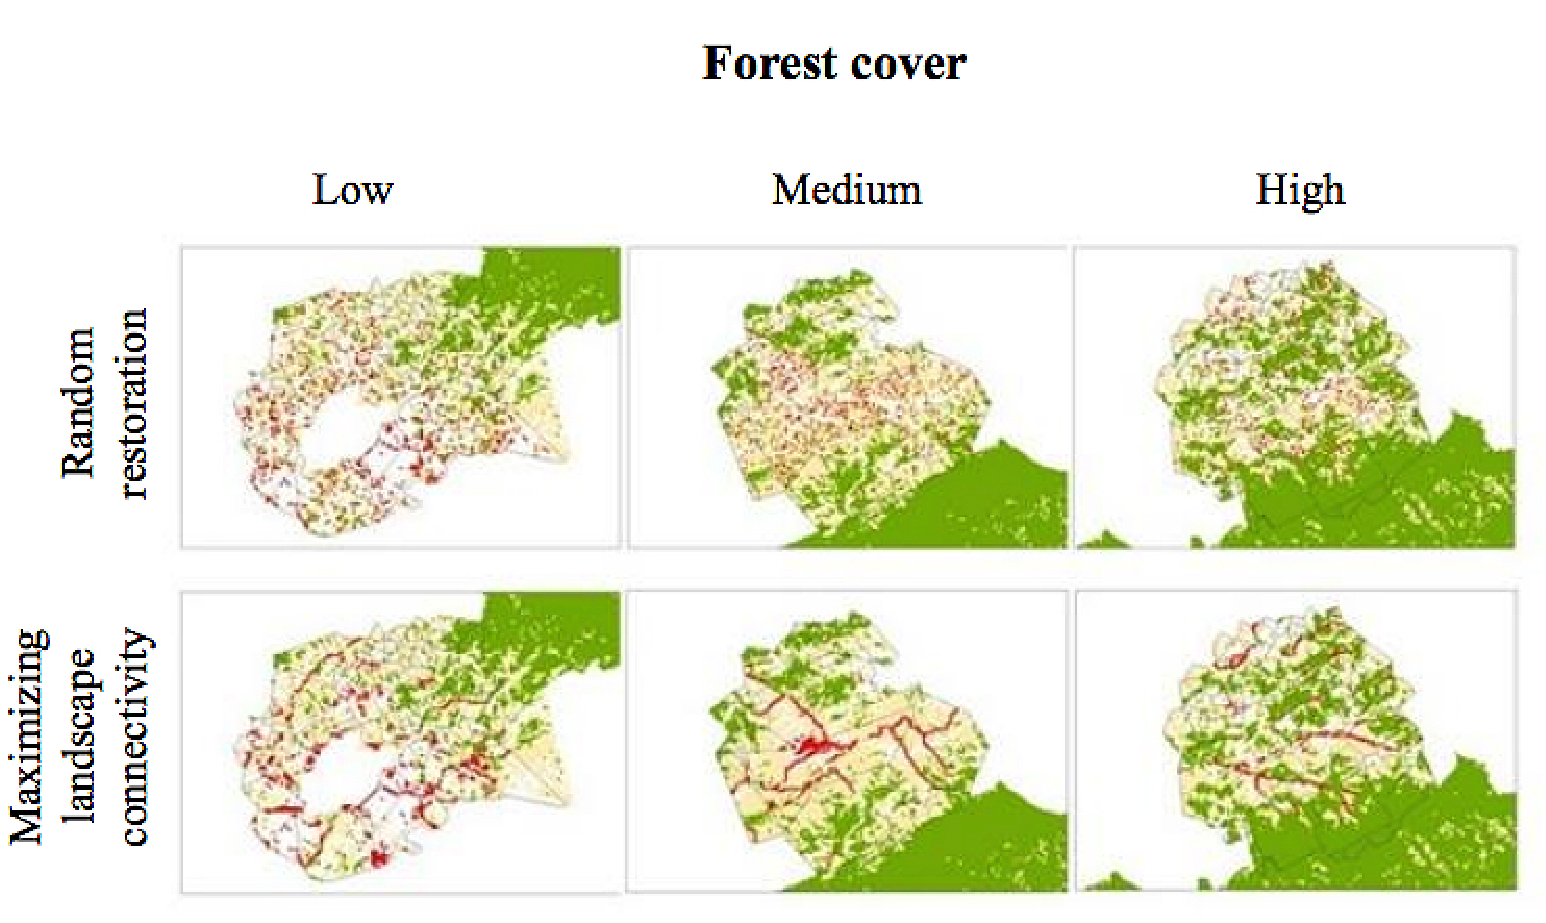
\includegraphics[width=1.0\linewidth]{pictureve/Bio-Renatinho-2.pdf}
\caption{Simulated restored areas based on the strategies targeting random restoration and maximizing landscape connectivity with landscapes with different amounts of forest cover: low (10\%), medium (30\%) and high (50\%). Green: current forest cover, Yellow: restorable areas (i.e. agriculture and pastureland), Red: restored forest cover after 20 years; and Blank: non-restorable areas (i.e. urban areas, rivers and roads). }
\label{fig:Bio-Renatinho-2}
\end{figure}

We reveal three main findings: i) restoration strategies that target for landscape connectivity can accelerate and anticipate biodiversity benefits of restoration initiatives, even when restoration is limited by spatial constrains (e.g. as specified by the NVPL); ii) the benefit of each restoration strategy will depend on both the amount of forest cover in the landscape  and the species dispersal ability; and iii) spatial planning increases effectiveness of restoration initiatives and their outcomes (e.g. biodiversity recovery). \\



%-----------------------------------------------------------------------------------------------


\section{\Large Extinction risk }\label{sec:bio-extinct}

Analyses that account for the probability of avoided extinctions can be a useful tool for subsidizing conservation and restoration policies and practices. To evaluate the effectiveness of a conservation intervention, it is desirable to consider whether the interventions are being able to avoid loss of ecosystems, species or any other valued aspects of the natural environment \citep{Pressey2015}. Most conservation interventions are usually placed in areas where they have least potential for making a difference in species persistence, such as areas suffering from low human pressures \citep{Andam2008}. Differently, landscape restoration initiatives are preferably placed in areas where it can yield the highest impacts on species conservation by, for example, reducing the probability of extinction of a species through restoration of landscapes within the species potential distribution \citep{Thomas2004, Strassburg0StrategicCosts}. In the FLR context, therefore, high-valued areas are those with the potential for delivering the highest number of avoided extinctions across multiple taxonomic groups. 
	
Here we measured the probability of extinction for endemic Atlantic Forest species as a function of the marginal contribution of each hectare restored to reducing species’ extinction probability \cite{Strassburg0StrategicCosts}. In this approach, the value of restoring additional habitat for a species diminishes as the total area of habitat increases. For example, if existing habitat area is small there is a large benefit to increasing that area through restoration, but as the area of habitat restored increases there is a diminishing benefit for the addition of more habitat area restored. We used the potential species distribution instead of the current species distribution because restoration would expand available habitat area for the species. This is different from the usual approach in conservation prioritization where the aim is to conserve current habitats by using species’ distribution that falls within native vegetation.

We generated potential species occurrence models for 2,392 species of plants (n = 2,046), birds (n = 223) and amphibians (n = 123) native to the Brazilian Atlantic Forest (Figure \ref{fig:Bio-Extinct-1}). The overlay of the potential distribution maps for all taxonomic groups shows that the highest species’ richness are found along the Brazilian coast, specially within the States of Rio de Janeiro, São Paulo, Paraná, Santa Catarina and Rio Grande do Sul, and also extending to inner regions of Minas Gerais in the transition to the Cerrado biome. From this set of species, 33\% (n = 785) are endemic to the biome and were used to calculate the avoided extinction risk (Figure \ref{fig:Bio-Extinct-2}).  \\
 
 \newpage
 %%%%%% FIgura Bio-Extinct-1 %%%%%%%% 
\begin{figure}[H]
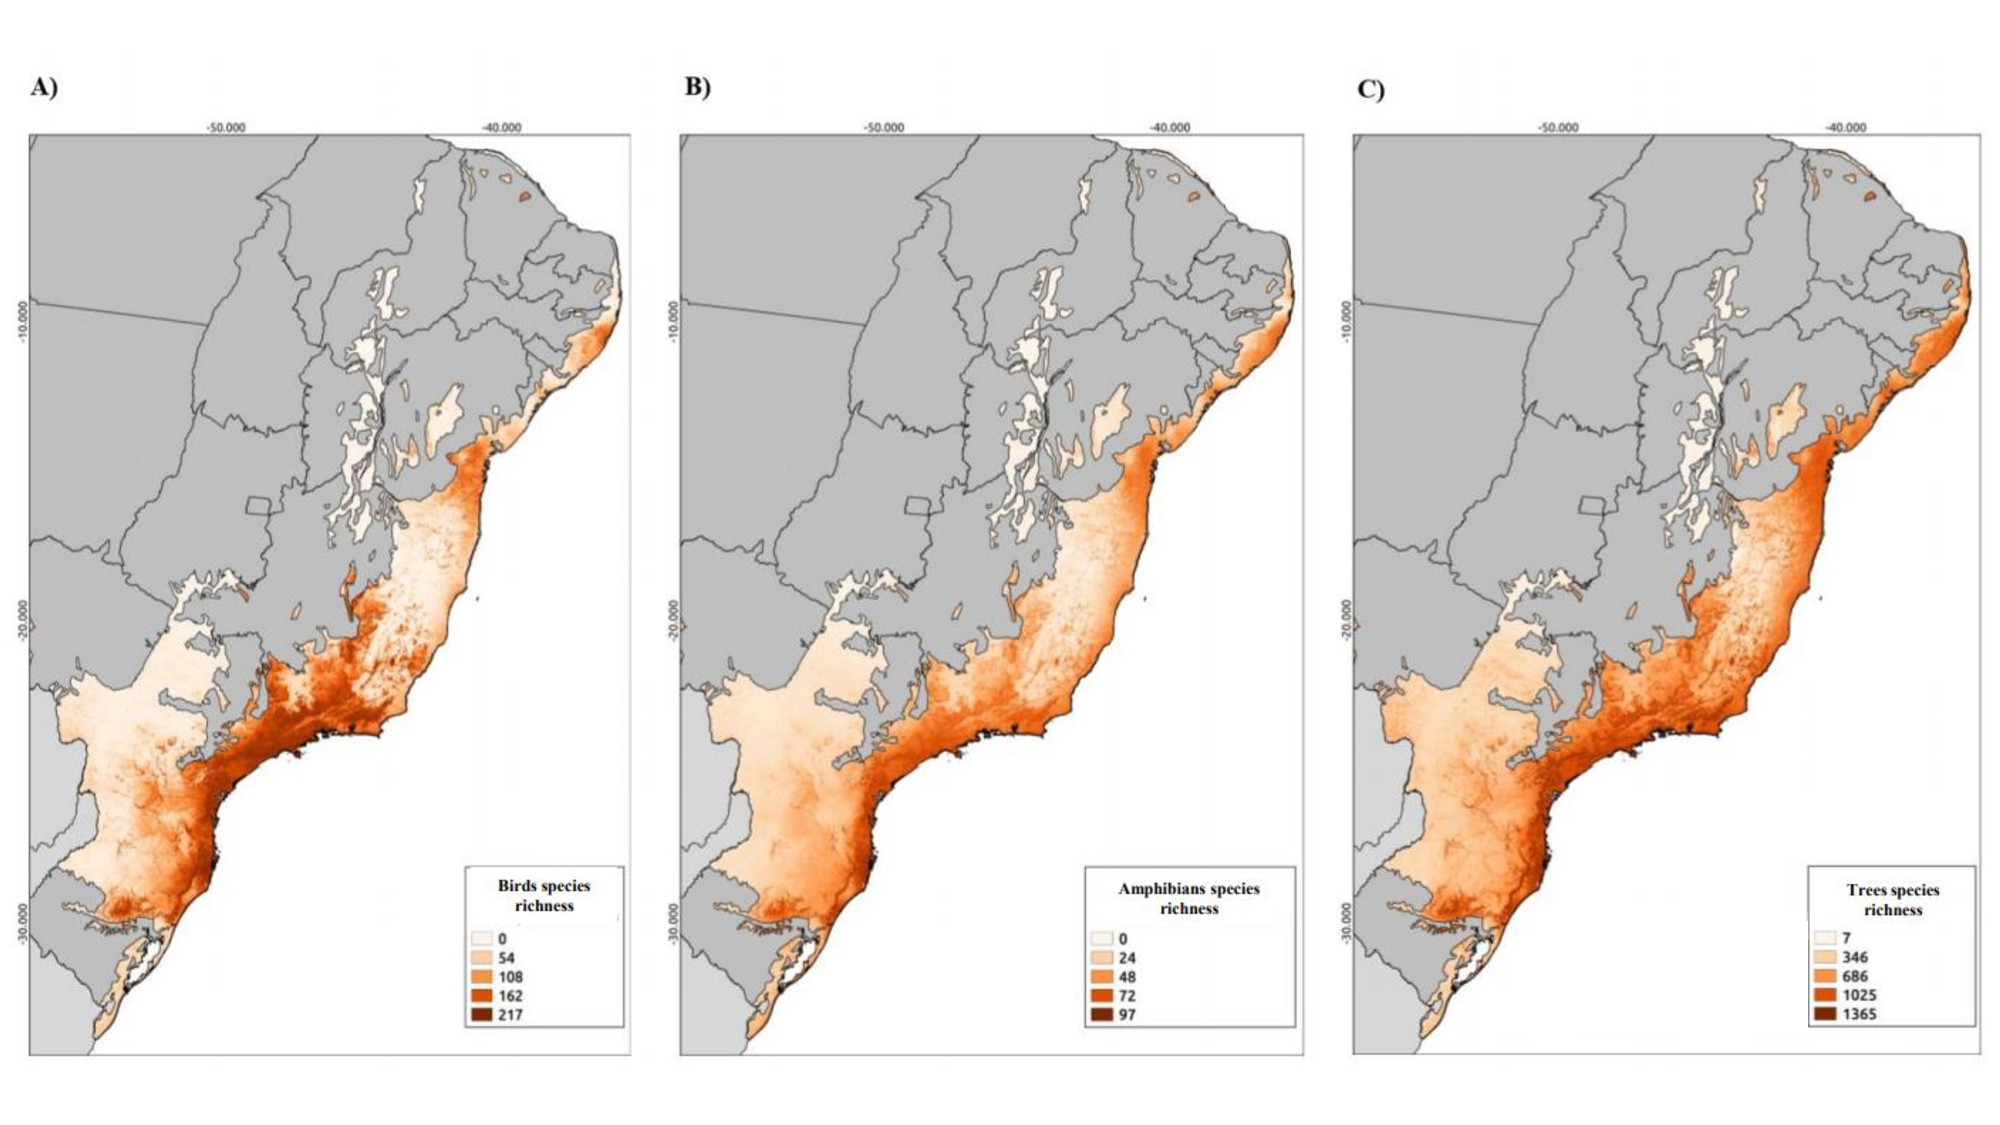
\includegraphics[width=1.0\linewidth]{pictureve/Bio-Extinct-1.pdf}
\caption{Potential species richness distribution across the Brazilian Atlantic Forest for (a) woody plants, (b) birds and (c) amphibians. The darker the colour the higher the species richness in the planning unit.}
\label{fig:Bio-Extinct-1}
\end{figure}
 
 %Figure 5. \textcolor{blue}{FIGURA-BIODIV-EXTINC-1.} Potential species richness distribution across the Brazilian Atlantic Forest for (a) woody plants, (b) birds and (c) amphibians. The darker the colour the higher the species richness in the planning unit. \\
 

We aggregated the avoided extinction risk at each planning unit across all endemic species, thereby generating a FLR biodiversity-benefits surface. Our results show that the highest number of avoided extinctions of endemic species (Figure \ref{fig:Bio-Extinct-2}) coincides with the areas holding the highest species richness in the biome (Figure \ref{fig:Bio-Extinct-1}). Despite less biodiverse, the northeastern Brazil would also greatly benefit from restoration, especially avoiding the extinction of bird and amphibian species. Restoration in the southeastern region of the State of Bahia, for example, would importantly reduce species extinction risk as it is considered a global hotspot of biodiversity, holding one of the highest levels of plant species richness in the world \citep{Thomas1998}, and being an important center of endemism for amphibians. FLR in these areas, which have been highly deforested in the past, would yield the highest benefits for biodiversity conservation and therefore should be prioritized when planning restoration aiming to conserve biodiversity.  \\

\newpage
 %%%%%% FIgura Bio-Extinct-2 %%%%%%%% 
\begin{figure}[H]
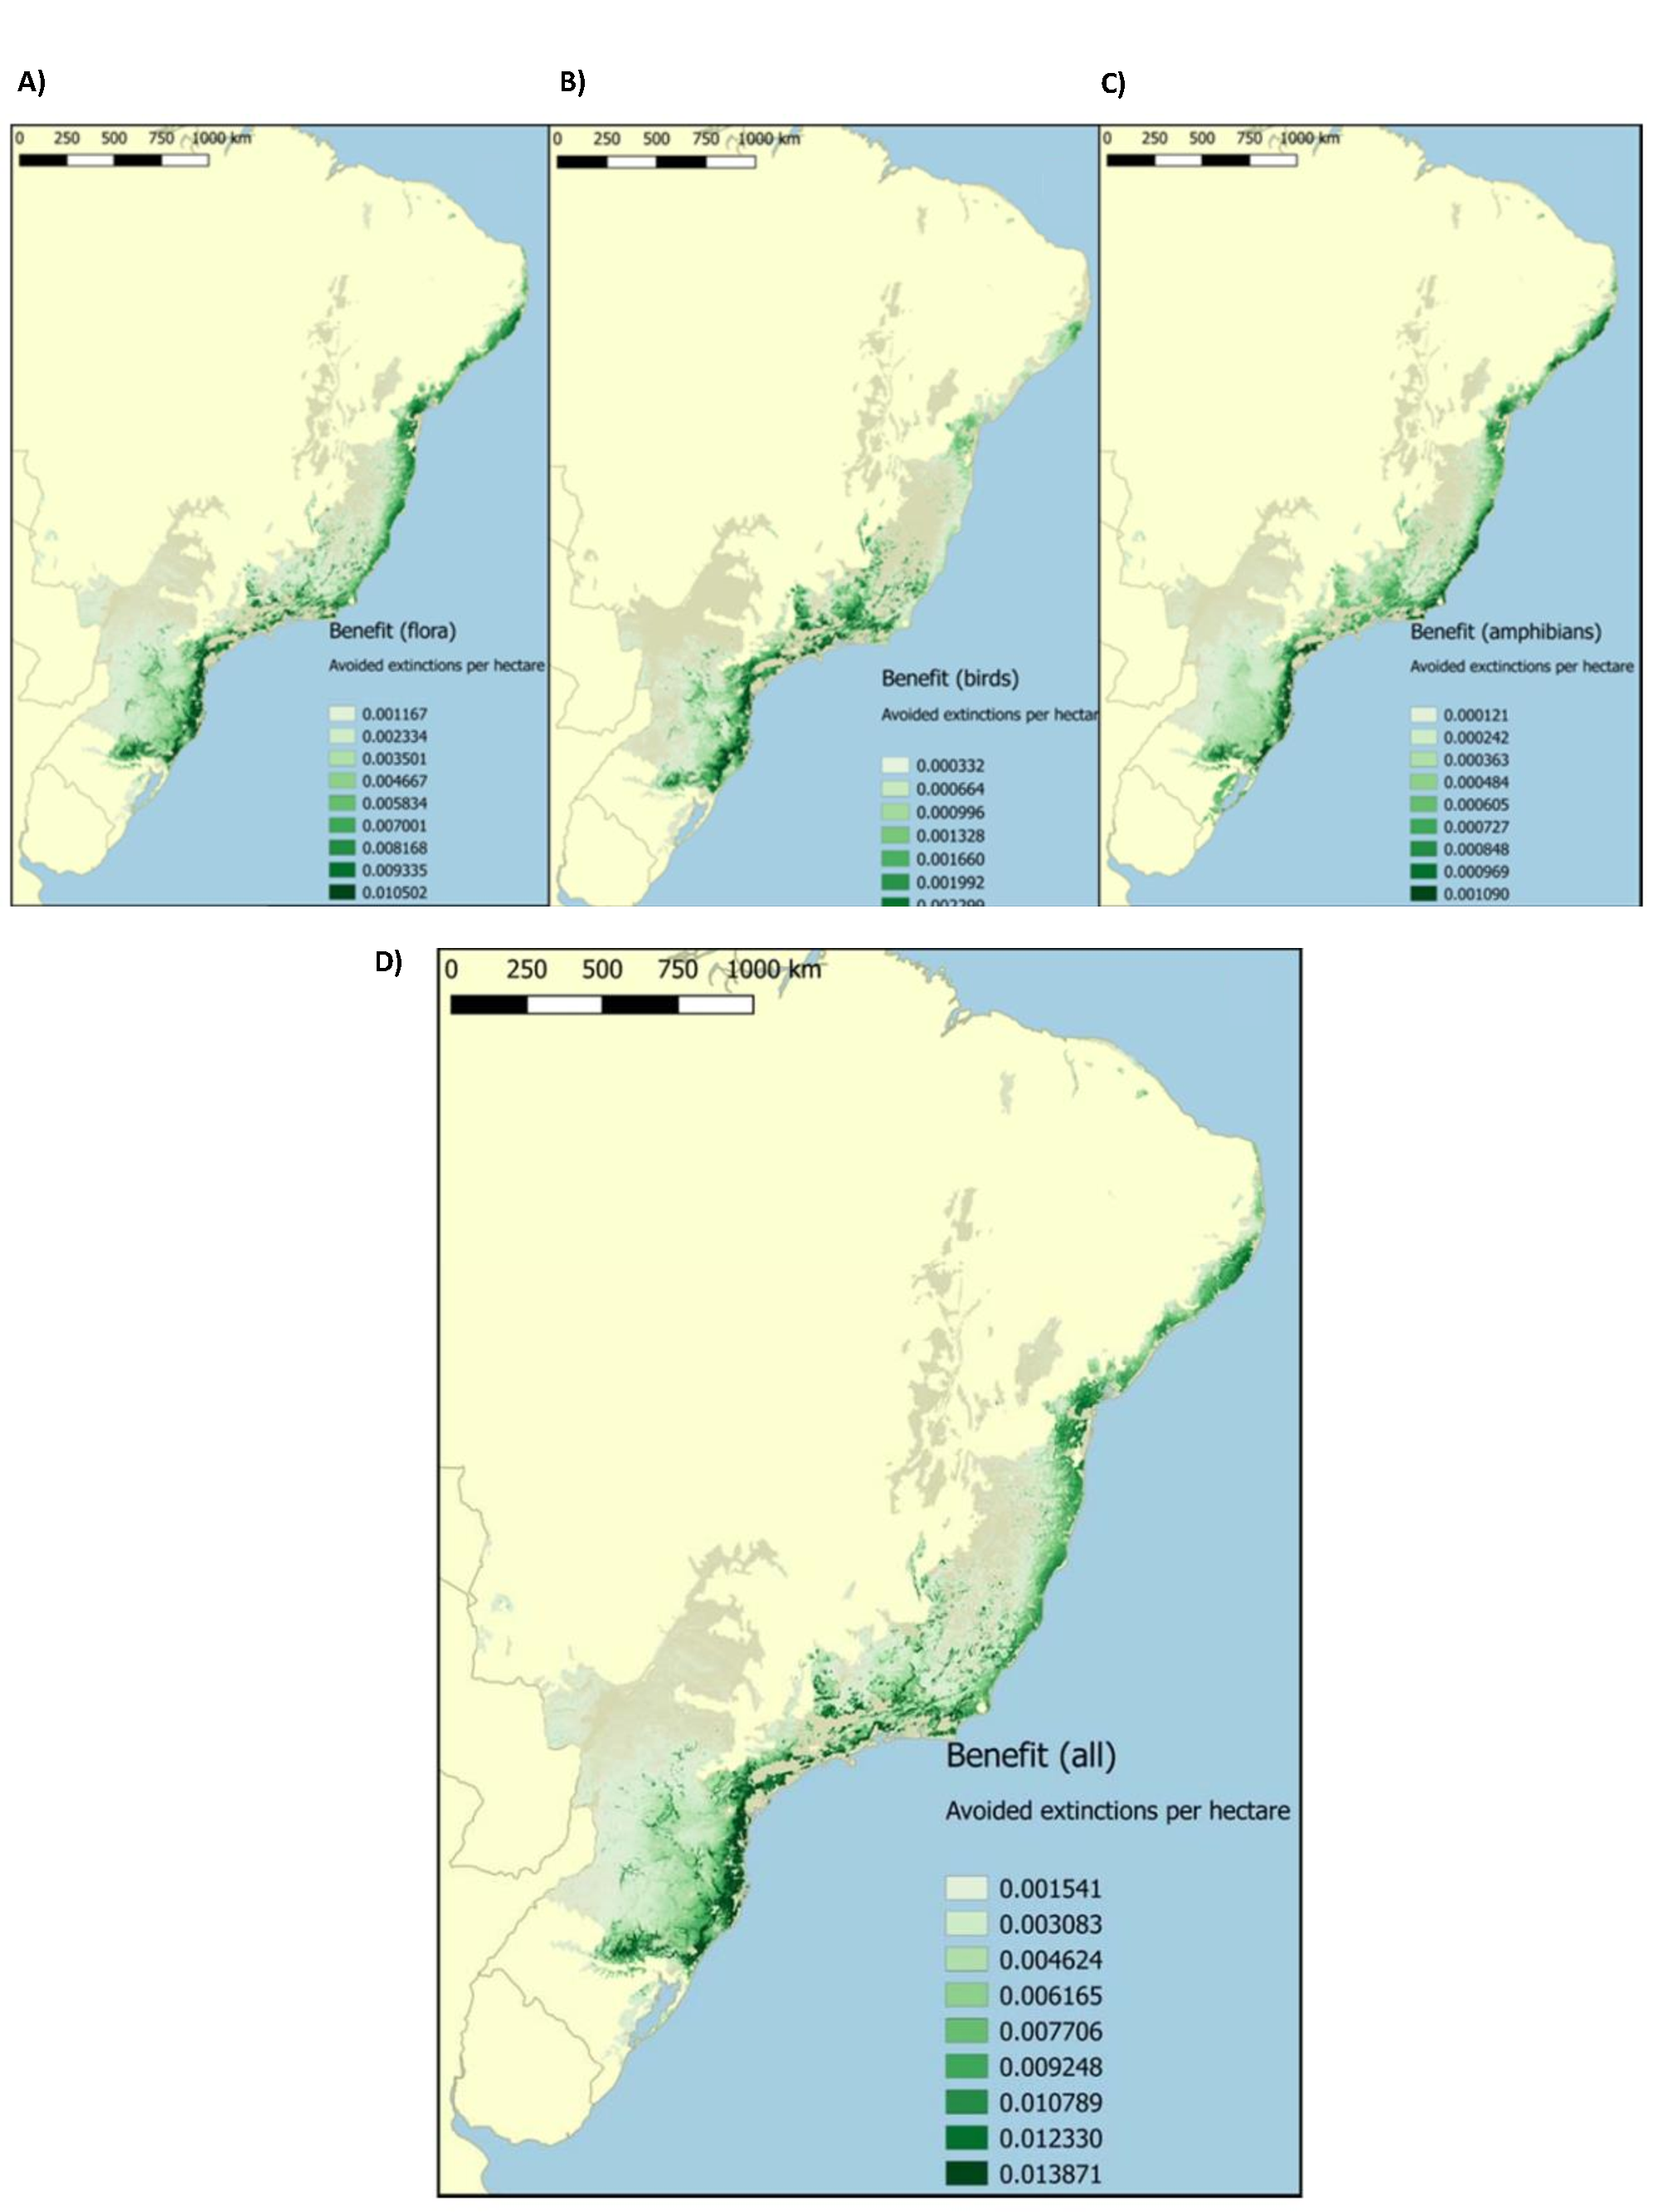
\includegraphics[width=1.0\linewidth]{pictureve/Bio-Extinct-2.pdf}
\caption{Surface of biodiversity conservation benefits from restoration for amphibians, birds, plants and all species combined. The benefits for biodiversity conservation was measured in terms of avoided extinctions per hectare, and the maps show these benefits for (a) woody plants, (b) birds, (c) amphibians and (d) for all species combined. Importantly, these benefits are shown here for the starting situation. As restoration occurs such pattern will change.}
\label{fig:Bio-Extinct-2}
\end{figure}

%Figure 6.\textcolor{blue}{FIGURA-BIODIV-EXTINC-2.} Surface of biodiversity conservation benefits from restoration for amphibians, birds, plants and all species combined. The benefits for biodiversity conservation was measured in terms of avoided extinctions per hectare, and the maps show these benefits for (a) woody plants, (b) birds, (c) amphibians and (d) for all species combined. Importantly, these benefits are shown here for the starting situation. As restoration occurs such pattern will change.\\






